\chapter*{Введение}                         % Заголовок
\addcontentsline{toc}{chapter}{Введение}    % Добавляем его в оглавление, если нет нумерации, то есть
%\chapter*{Введение}

\newcommand{\actuality}{}
\newcommand{\progress}{}
\newcommand{\aim}{{\textbf\aimTXT}}
\newcommand{\tasks}{\textbf{\tasksTXT}}
%\newcommand{\novelty}{\textbf{\noveltyTXT}}
\newcommand{\influence}{\textbf{\influenceTXT}}
\newcommand{\methods}{\textbf{\methodsTXT}}
\newcommand{\defpositions}{\textbf{\defpositionsTXT}}
\newcommand{\reliability}{\textbf{\reliabilityTXT}}
\newcommand{\probation}{\textbf{\probationTXT}}
\newcommand{\contribution}{\textbf{\contributionTXT}}
\newcommand{\publications}{\textbf{\publicationsTXT}}

%
{\actuality} Обзор, введение в тему, обозначение места данной работы в
мировых исследованиях и~т.\:п., можно использовать ссылки на~другие
работы\ifnumequal{\value{bibliosel}}{1}{~\autocite{Gosele1999161}}{}
(если их~нет, то~в~автореферате
автоматически пропадёт раздел <<Список литературы>>). Внимание! Ссылки
на~другие работы в разделе общей характеристики работы можно
использовать только при использовании \verb!biblatex! (из-за технических
ограничений \verb!bibtex8!. Это связано с тем, что одна
и~та~же~характеристика используются и~в~тексте диссертации, и в
автореферате. В~последнем, согласно ГОСТ, должен присутствовать список
работ автора по~теме диссертации, а~\verb!bibtex8! не~умеет выводить в одном
файле два списка литературы).
При использовании \verb!biblatex! возможно использование исключительно
в~автореферате подстрочных ссылок
для других работ командой \verb!\autocite!, а~также цитирование
собственных работ командой \verb!\cite!. Для этого в~файле
\verb!Synopsis/setup.tex! необходимо присвоить положительное значение
счётчику \verb!\setcounter{usefootcite}{1}!.

Для генерации содержимого титульного листа автореферата, диссертации
и~презентации используются данные из файла \verb!common/data.tex!. Если,
например, вы меняете название диссертации, то оно автоматически
появится в~итоговых файлах после очередного запуска \LaTeX. Согласно
ГОСТ 7.0.11-2011 <<5.1.1 Титульный лист является первой страницей
диссертации, служит источником информации, необходимой для обработки и
поиска документа>>. Наличие логотипа организации на~титульном листе
упрощает обработку и~поиск, для этого разметите логотип вашей
организации в папке images в~формате PDF (лучше найти его в векторном
варианте, чтобы он хорошо смотрелся при печати) под именем
\verb!logo.pdf!. Настроить размер изображения с логотипом можно
в~соответствующих местах файлов \verb!title.tex!  отдельно для
диссертации и автореферата. Если вам логотип не~нужен, то просто
удалите файл с~логотипом.

\ifsynopsis
Этот абзац появляется только в~автореферате.
Для формирования блоков, которые будут обрабатываться только в~автореферате,
заведена проверка условия \verb!\!\verb!ifsynopsis!.
Значение условия задаётся в~основном файле документа (\verb!synopsis.tex! для
автореферата).
\else
Этот абзац появляется только в~диссертации.
Через проверку условия \verb!\!\verb!ifsynopsis!, задаваемого в~основном файле
документа (\verb!dissertation.tex! для диссертации), можно сделать новую
команду, обеспечивающую появление цитаты в~диссертации, но~не~в~автореферате.
\fi

% {\progress} 
% Этот раздел должен быть отдельным структурным элементом по
% ГОСТ, но он, как правило, включается в описание актуальности
% темы. Нужен он отдельным структурынм элемементом или нет ---
% смотрите другие диссертации вашего совета, скорее всего не нужен.

{\aim} данной работы является \ldots

Для~достижения поставленной цели необходимо было решить следующие {\tasks}:
\begin{enumerate}
  \item Исследовать, разработать, вычислить и~т.\:д. и~т.\:п.
  \item Исследовать, разработать, вычислить и~т.\:д. и~т.\:п.
  \item Исследовать, разработать, вычислить и~т.\:д. и~т.\:п.
  \item Исследовать, разработать, вычислить и~т.\:д. и~т.\:п.
\end{enumerate}


{\novelty}
\begin{enumerate}
  \item Впервые \ldots
  \item Впервые \ldots
  \item Было выполнено оригинальное исследование \ldots
\end{enumerate}

{\influence} \ldots

{\methods} \ldots

{\defpositions}
\begin{enumerate}
  \item Первое положение
  \item Второе положение
  \item Третье положение
  \item Четвертое положение
\end{enumerate}
В папке Documents можно ознакомиться в решением совета из Томского ГУ
в~файле \verb+Def_positions.pdf+, где обоснованно даются рекомендации
по~формулировкам защищаемых положений. 

{\reliability} полученных результатов обеспечивается \ldots \ Результаты находятся в соответствии с результатами, полученными другими авторами.


{\probation}
Основные результаты работы докладывались~на:
перечисление основных конференций, симпозиумов и~т.\:п.

{\contribution} Автор принимал активное участие \ldots

%\publications\ Основные результаты по теме диссертации изложены в ХХ печатных изданиях~\cite{Sokolov,Gaidaenko,Lermontov,Management},
%Х из которых изданы в журналах, рекомендованных ВАК~\cite{Sokolov,Gaidaenko}, 
%ХХ --- в тезисах докладов~\cite{Lermontov,Management}.

\ifnumequal{\value{bibliosel}}{0}{% Встроенная реализация с загрузкой файла через движок bibtex8
    \publications\ Основные результаты по теме диссертации изложены в XX печатных изданиях, 
    X из которых изданы в журналах, рекомендованных ВАК, 
    X "--- в тезисах докладов.%
}{% Реализация пакетом biblatex через движок biber
%Сделана отдельная секция, чтобы не отображались в списке цитированных материалов
    \begin{refsection}[vak,papers,conf]% Подсчет и нумерация авторских работ. Засчитываются только те, которые были прописаны внутри \nocite{}.
        %Чтобы сменить порядок разделов в сгрупированном списке литературы необходимо перетасовать следующие три строчки, а также команды в разделе \newcommand*{\insertbiblioauthorgrouped} в файле biblio/biblatex.tex
        \printbibliography[heading=countauthorvak, env=countauthorvak, keyword=biblioauthorvak, section=1]%
        \printbibliography[heading=countauthorconf, env=countauthorconf, keyword=biblioauthorconf, section=1]%
        \printbibliography[heading=countauthornotvak, env=countauthornotvak, keyword=biblioauthornotvak, section=1]%
        \printbibliography[heading=countauthor, env=countauthor, keyword=biblioauthor, section=1]%
        \nocite{%Порядок перечисления в этом блоке определяет порядок вывода в списке публикаций автора
                vakbib1,vakbib2,%
                confbib1,confbib2,%
                bib1,bib2,%
        }%
        \publications\ Основные результаты по теме диссертации изложены в~\arabic{citeauthor}~печатных изданиях, 
        \arabic{citeauthorvak} из которых изданы в журналах, рекомендованных ВАК, 
        \arabic{citeauthorconf} "--- в~тезисах докладов.
    \end{refsection}
    \begin{refsection}[vak,papers,conf]%Блок, позволяющий отобрать из всех работ автора наиболее значимые, и только их вывести в автореферате, но считать в блоке выше общее число работ
        \printbibliography[heading=countauthorvak, env=countauthorvak, keyword=biblioauthorvak, section=2]%
        \printbibliography[heading=countauthornotvak, env=countauthornotvak, keyword=biblioauthornotvak, section=2]%
        \printbibliography[heading=countauthorconf, env=countauthorconf, keyword=biblioauthorconf, section=2]%
        \printbibliography[heading=countauthor, env=countauthor, keyword=biblioauthor, section=2]%
        \nocite{vakbib2}%vak
        \nocite{bib1}%notvak
        \nocite{confbib1}%conf
    \end{refsection}
}
При использовании пакета \verb!biblatex! для автоматического подсчёта
количества публикаций автора по теме диссертации, необходимо
их~здесь перечислить с использованием команды \verb!\nocite!.
 % Характеристика работы по структуре во введении и в автореферате не отличается (ГОСТ Р 7.0.11, пункты 5.3.1 и 9.2.1), потому её загружаем из одного и того же внешнего файла, предварительно задав форму выделения некоторым параметрам

%\textbf{Объем и структура работы.} Диссертация состоит из~введения, трёх глав,
%заключения и~двух приложений.
%% на случай ошибок оставляю исходный кусок на месте, закомментированным
%Полный объём диссертации составляет  \ref*{TotPages}~страницу
%с~\totalfigures{}~рисунками и~\totaltables{}~таблицами. Список литературы
%содержит \total{citenum}~наименований.
%
%Полный объём диссертации составляет
%\formbytotal{TotPages}{страниц}{у}{ы}{}, включая
%\formbytotal{totalcount@figure}{рисун}{ок}{ка}{ков} и
%\formbytotal{totalcount@table}{таблиц}{у}{ы}{}.   Список литературы содержит
%\formbytotal{citenum}{наименован}{ие}{ия}{ий}.

\noindent

\begin{figure}[!h]
	\centering
  \tikzset{every picture/.style={line width=0.75pt}} %set default line width to 0.75pt

  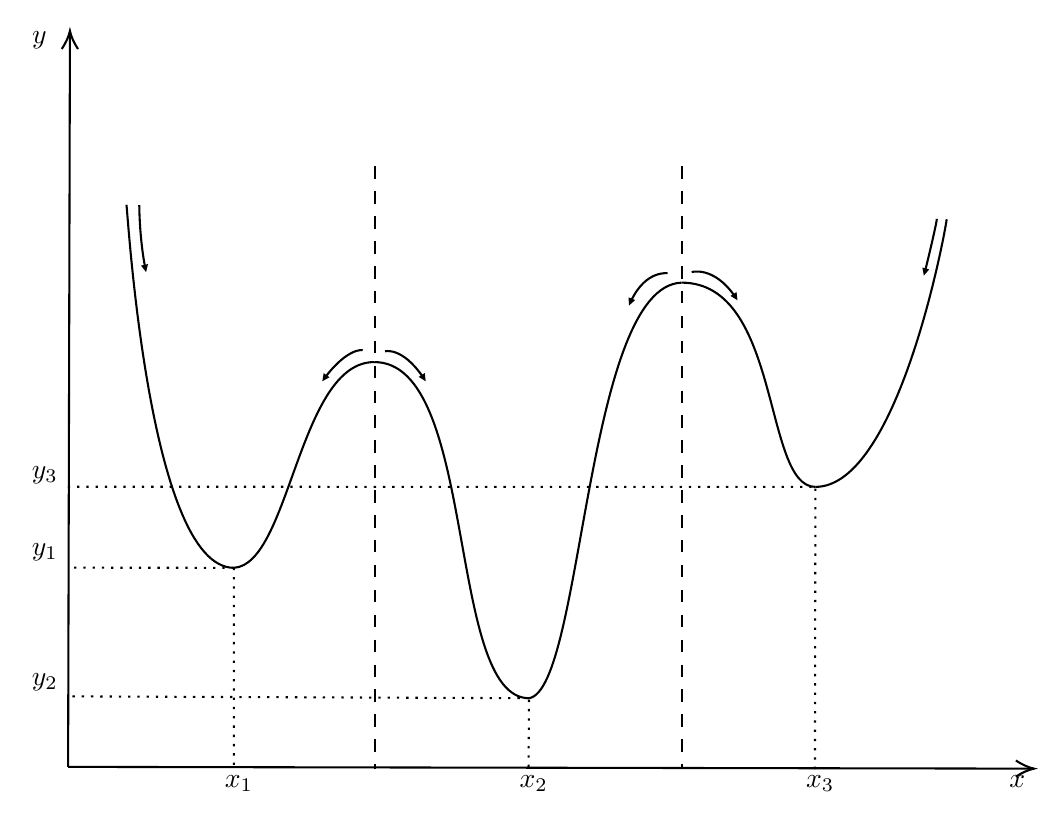
\begin{tikzpicture}[x=0.75pt,y=0.75pt,yscale=-1,xscale=1]
  %uncomment if require: \path (0,601); %set diagram left start at 0, and has height of 601

  %Curve Lines [id:da37232558430014473]
  \draw    (196.17,196.94) .. controls (246.25,196.85) and (230.73,358.89) .. (270.74,358.89) ;
  %Straight Lines [id:da3476897261424843]
  \draw    (48.67,391.97) -- (49.55,39.36) ;
  \draw [shift={(49.55,37.36)}, rotate = 450.14] [color={rgb, 255:red, 0; green, 0; blue, 0 }  ][line width=0.75]    (8.74,-3.92) .. controls (5.56,-1.84) and (2.65,-0.53) .. (0,0) .. controls (2.65,0.53) and (5.56,1.84) .. (8.74,3.92)   ;
  %Straight Lines [id:da355319366378235]
  \draw    (48.67,391.97) -- (512.03,392.82) ;
  \draw [shift={(514.03,392.82)}, rotate = 180.1] [color={rgb, 255:red, 0; green, 0; blue, 0 }  ][line width=0.75]    (8.74,-3.92) .. controls (5.56,-1.84) and (2.65,-0.53) .. (0,0) .. controls (2.65,0.53) and (5.56,1.84) .. (8.74,3.92)   ;
  %Curve Lines [id:da9451459693396738]
  \draw    (128.57,296.07) .. controls (155.62,294.41) and (159.71,196.85) .. (196.17,196.94) ;
  %Curve Lines [id:da9118683996504104]
  \draw    (270.74,358.89) .. controls (296.86,354.64) and (297.68,160.37) .. (344.22,158.67) ;
  %Curve Lines [id:da2198725124040073]
  \draw    (128.57,296.07) .. controls (87.05,296.11) and (77.25,121.35) .. (76.77,121.18) ;
  %Curve Lines [id:da7607618362532125]
  \draw    (408.71,257.08) .. controls (383.4,257.08) and (392.38,158.67) .. (344.22,158.67) ;
  %Curve Lines [id:da5694398882679776]
  \draw    (471.93,128.13) .. controls (472.39,128.13) and (449.53,257.08) .. (408.71,257.08) ;
  %Straight Lines [id:da9091864738783852]
  \draw  [dash pattern={on 4.5pt off 4.5pt}]  (196.44,102.68) -- (196.44,392.82) ;
  %Straight Lines [id:da6947024773973995]
  \draw  [dash pattern={on 4.5pt off 4.5pt}]  (344.22,102.68) -- (344.22,392.82) ;
  %Curve Lines [id:da3791802319426323]
  \draw [line width=0.75]    (82.96,121.35) .. controls (82.96,121.35) and (82.96,136.34) .. (85.68,150.82) ;
  \draw [shift={(86.23,153.58)}, rotate = 257.93] [fill={rgb, 255:red, 0; green, 0; blue, 0 }  ][line width=0.08]  [draw opacity=0] (3.57,-1.72) -- (0,0) -- (3.57,1.72) -- cycle    ;
  %Curve Lines [id:da6195588467790258]
  \draw [line width=0.75]    (190.54,191.34) .. controls (190.72,190.93) and (183.36,190.15) .. (172.83,203.89) ;
  \draw [shift={(171.14,206.18)}, rotate = 305.34000000000003] [fill={rgb, 255:red, 0; green, 0; blue, 0 }  ][line width=0.08]  [draw opacity=0] (3.57,-1.72) -- (0,0) -- (3.57,1.72) -- cycle    ;
  %Curve Lines [id:da8600369809168591]
  \draw [line width=0.75]    (467.22,127.96) .. controls (467.22,129.38) and (463.73,144.47) .. (461.7,152.46) ;
  \draw [shift={(460.96,155.28)}, rotate = 285.23] [fill={rgb, 255:red, 0; green, 0; blue, 0 }  ][line width=0.08]  [draw opacity=0] (3.57,-1.72) -- (0,0) -- (3.57,1.72) -- cycle    ;
  %Curve Lines [id:da2891730950552185]
  \draw [line width=0.75]    (201.34,191.76) .. controls (201.34,191.76) and (209.45,189.46) .. (219.36,203.78) ;
  \draw [shift={(220.94,206.18)}, rotate = 237.97] [fill={rgb, 255:red, 0; green, 0; blue, 0 }  ][line width=0.08]  [draw opacity=0] (3.57,-1.72) -- (0,0) -- (3.57,1.72) -- cycle    ;
  %Curve Lines [id:da17721713207409828]
  \draw [line width=0.75]    (337.49,154.01) .. controls (337.67,154.41) and (327.37,152.13) .. (320.04,167.18) ;
  \draw [shift={(318.91,169.7)}, rotate = 292.40999999999997] [fill={rgb, 255:red, 0; green, 0; blue, 0 }  ][line width=0.08]  [draw opacity=0] (3.57,-1.72) -- (0,0) -- (3.57,1.72) -- cycle    ;
  %Curve Lines [id:da026627679148430117]
  \draw [line width=0.75]    (349.11,153.58) .. controls (349.11,153.58) and (359.43,150.52) .. (369.56,164.76) ;
  \draw [shift={(371.16,167.16)}, rotate = 237.97] [fill={rgb, 255:red, 0; green, 0; blue, 0 }  ][line width=0.08]  [draw opacity=0] (3.57,-1.72) -- (0,0) -- (3.57,1.72) -- cycle    ;
  %Straight Lines [id:da6295058967697196]
  \draw  [dash pattern={on 0.84pt off 2.51pt}]  (128.57,296.07) -- (128.5,394) ;
  %Straight Lines [id:da21636754919622114]
  \draw  [dash pattern={on 0.84pt off 2.51pt}]  (128.57,296.07) -- (48.5,296) ;
  %Straight Lines [id:da2606087008268614]
  \draw  [dash pattern={on 0.84pt off 2.51pt}]  (270.74,358.89) -- (49.5,358) ;
  %Straight Lines [id:da4174193236101569]
  \draw  [dash pattern={on 0.84pt off 2.51pt}]  (270.5,392) -- (270.74,358.89) ;
  %Straight Lines [id:da5819250360910133]
  \draw  [dash pattern={on 0.84pt off 2.51pt}]  (408.5,393) -- (408.71,257.08) ;
  %Straight Lines [id:da5898884588834679]
  \draw  [dash pattern={on 0.84pt off 2.51pt}]  (48.5,257) -- (408.71,257.08) ;

  % Text Node
  \draw (500.69,394.67) node [anchor=north west][inner sep=0.75pt]   [align=left] {$\displaystyle x$};
  % Text Node
  \draw (29.81,36.33) node [anchor=north west][inner sep=0.75pt]   [align=left] {$\displaystyle y$};
  % Text Node
  \draw (402.69,394.67) node [anchor=north west][inner sep=0.75pt]   [align=left] {$\displaystyle x_{3}$};
  % Text Node
  \draw (264.69,394.67) node [anchor=north west][inner sep=0.75pt]   [align=left] {$\displaystyle x_{2}$};
  % Text Node
  \draw (122.69,394.67) node [anchor=north west][inner sep=0.75pt]   [align=left] {$\displaystyle x_{1}$};
  % Text Node
  \draw (29.69,282.67) node [anchor=north west][inner sep=0.75pt]   [align=left] {$\displaystyle y_{1}$};
  % Text Node
  \draw (29.69,345.67) node [anchor=north west][inner sep=0.75pt]   [align=left] {$\displaystyle y_{2}$};
  % Text Node
  \draw (29.69,245.67) node [anchor=north west][inner sep=0.75pt]   [align=left] {$\displaystyle y_{3}$};


  \end{tikzpicture}

	\label{img:example}
\end{figure}
